\section{Podłączenie do Sieci Internet za Pomocą Łącza}
\subsection{Wybór Dostawcy Usługi Łącza Satelitarnego}
    Wybór padł na firmę StarLink.
    
\includegraphics[width=0.3\textwidth]{3-starlink.png}
\subsection{Opis Rozwiązania Dostawcy}
    Ten wysokowydajny zestaw jest najlepszy dla zaawansowanych użytkowników i zastosowań
    korporacyjnych. Zestaw Flat High Performance zawiera wszystko, co potrzebne do uzyskania
    połączenia z internetem. Dodatkowe parametry wykraczające poza zestaw standardowy:
    \begin{itemize}
        \item Łatwa integracja z siecią
        \item Możliwość podłączenia własnego routera bezpośrednio do anteny przez port Ethernet
        \item Lepsza odporność na warunki pogodowe
        \item 3x razy większa prędkość przy >35°C (95°F)
        \item 1,7x lepsza zdolność topienia śniegu
        \item Lepszy stosunek sygnału do szumu skutkujący dłuższym czasem pracy podczas burzy
        \item Zwiększona odporność
        \item Większa widoczność satelitarna dla optymalnego czasu pracy
    \end{itemize}
\subsection{Specyfikacja Techniczna Łącza Satelitarnego}
\begin{flushleft}
    \begin{table}[h]
        \renewcommand{\arraystretch}{1.5}
        \begin{tabular}{|l|l|}
            \hline
            \textbf{Parametr} & \textbf{Wartość} \\
            \hline
            Pobieranie & 40-220+ MB/s \\
            Przesyłanie & 8-25+ MB/s \\
            Opóźnienie & 25-60 ms/s \\
            \hline
        \end{tabular}
        \caption{Dane dotyczące transferu danych}
    \end{table}
\end{flushleft}


\subsection{Schemat Logiczny Podłączenia do Sieci Internet}
    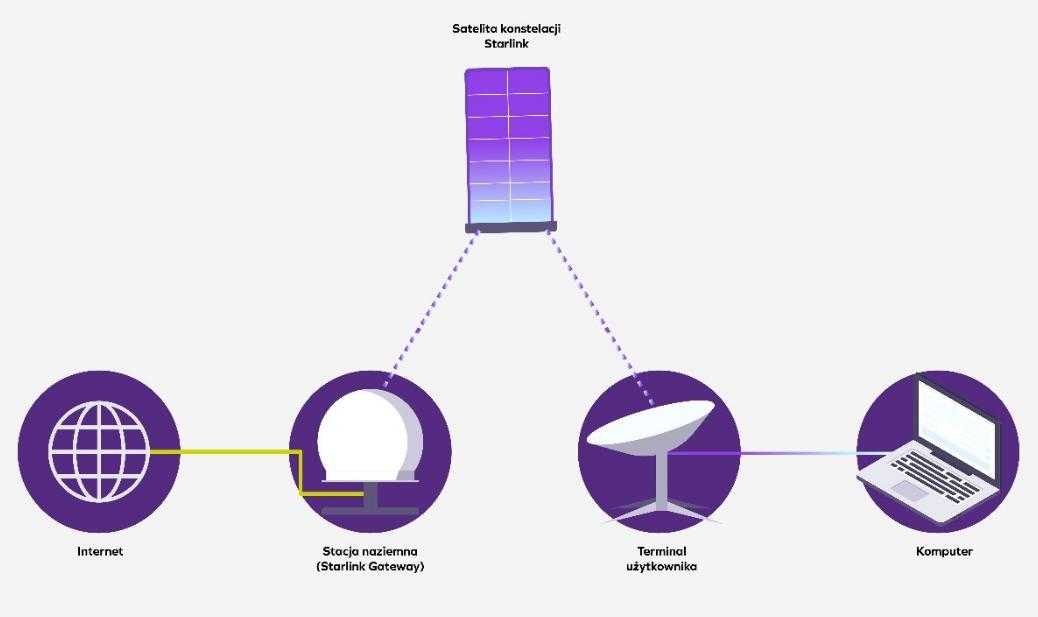
\includegraphics[width=0.8\textwidth]{4-schemat.jpg}


\subsection{Kosztorys Podłączenia do Sieci Satelitarnej}
    \begin{flushleft}
        \begin{table}[h]
            \renewcommand{\arraystretch}{1.5}
            \begin{tabular}{|l|l|}
                \hline
                \textbf{Cena za sprzęt odbiorczy} & 13 600,11 \\
                \hline
                \textbf{Cena abonamentu miesięcznego} & 6 051,60 zł \\
                \hline
            \end{tabular}
        \end{table}
    \end{flushleft}


